% Architecture figure for sec:method-architecture.
% Frozen LLM as shared encoder/generator; adapter MLP; three trainable heads.
%
% Conventions:
%   - Trainable components: light blue fill, solid border.
%   - Frozen components:    white fill, thick solid border, "(frozen)".
%   - Solid arrows:         data flow.
%   - Dashed arrow:         KV-cache reuse (LLM embedding pass to the
%                           verb-instantiator continuation).

\usetikzlibrary{positioning, arrows.meta, shapes.geometric, fit, calc,
                backgrounds}

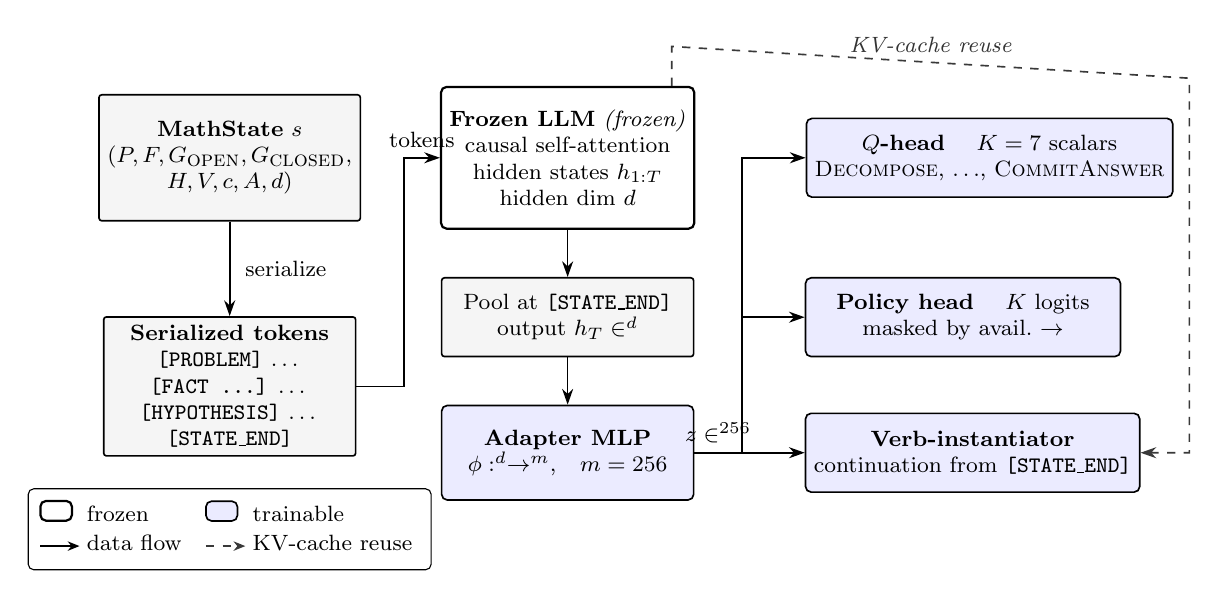
\begin{tikzpicture}[
  font=\footnotesize,
  >={Stealth[length=2mm, width=1.4mm]},
  every node/.style={align=center},
  frozen/.style={
    draw, thick, rectangle, rounded corners=2pt,
    fill=white,
    inner sep=3pt
  },
  trainable/.style={
    draw, semithick, rectangle, rounded corners=2pt,
    fill=blue!8,
    inner sep=3pt
  },
  data/.style={
    draw, semithick, rectangle, rounded corners=1pt,
    fill=gray!8,
    inner sep=3pt
  },
  head/.style={
    draw, semithick, rectangle, rounded corners=2pt,
    fill=blue!8,
    minimum width=40mm,
    minimum height=10mm,
    inner sep=3pt
  },
  flow/.style={->, semithick},
  cache/.style={->, dashed, semithick, gray!45!black},
]

% =====================================================================
% Left column: input and serialized tokens (stacked vertically)
% =====================================================================
\node[data, minimum width=32mm, minimum height=16mm] (state) {%
  \textbf{MathState} $s$\\
  $(P, F, G_{\textsc{open}}, G_{\textsc{closed}},$\\
  $H, V, c, A, d)$
};

\node[data, below=12mm of state, minimum width=32mm, minimum height=16mm]
  (tokens) {%
  \textbf{Serialized tokens}\\
  \texttt{[PROBLEM]} \ldots\\
  \texttt{[FACT \ldots]} \ldots\\
  \texttt{[HYPOTHESIS]} \ldots\\
  \texttt{[STATE\_END]}
};

% =====================================================================
% Center column: LLM, then pool, then adapter (vertical stack)
% =====================================================================
\node[frozen, right=10mm of state,
      minimum width=32mm, minimum height=18mm] (llm) {%
  \textbf{Frozen LLM} \emph{(frozen)}\\
  causal self-attention\\
  hidden states $h_{1{:}T}$\\
  hidden dim $d$
};

\node[data, below=6mm of llm,
      minimum width=32mm, minimum height=10mm] (pool) {%
  Pool at \texttt{[STATE\_END]}\\
  output $h_T \in \R^{d}$
};

\node[trainable, below=6mm of pool,
      minimum width=32mm, minimum height=12mm] (adapter) {%
  \textbf{Adapter MLP}\\
  $\phi: \R^{d} \to \R^{m}$,\quad $m = 256$
};

% =====================================================================
% Right column: three heads, stacked vertically
% =====================================================================
\node[head, right=14mm of llm] (qhead) {%
  \textbf{$Q$-head} \quad $K = 7$ scalars\\
  \textsc{Decompose}, $\ldots$, \textsc{CommitAnswer}
};

\node[head, right=14mm of pool] (polhead) {%
  \textbf{Policy head} \quad $K$ logits\\
  masked by avail.\ $\to \softmax$
};

\node[head, right=14mm of adapter] (vihead) {%
  \textbf{Verb-instantiator}\\
  continuation from \texttt{[STATE\_END]}
};

% =====================================================================
% Arrows
% =====================================================================
% Left vertical flow
\draw[flow] (state) -- (tokens)
  node[midway, right=2pt]{$\mathrm{serialize}$};

% Tokens to LLM (sweeps right and up)
\draw[flow] (tokens.east) -- ++(6mm, 0) |- (llm.west)
  node[pos=0.75, above]{tokens};

% Central column vertical flow
\draw[flow] (llm.south) -- (pool.north);
\draw[flow] (pool.south) -- (adapter.north);

% Adapter fans right to all three heads via a vertical bus
\coordinate (fanBase) at ($(adapter.east) + (6mm, 0)$);
\draw[semithick] (adapter.east) -- (fanBase)
  node[midway, above]{$z \in \R^{256}$};
\draw[flow] (fanBase) |- (qhead.west);
\draw[flow] (fanBase) |- (polhead.west);
\draw[flow] (fanBase) |- (vihead.west);

% KV-cache reuse: dashed arrow from LLM directly to verb-instantiator.
% Routes above all three heads then drops down on the right-hand side,
% terminating at the right edge of the verb-instantiator box.
\coordinate (kvOut)  at ($(llm.north east) + (-3mm, 0)$);
\coordinate (kvTopL) at ($(kvOut) + (0, 5mm)$);
\coordinate (kvTopR) at ($(qhead.north east) + (2mm, 5mm)$);
\coordinate (kvDrop) at ($(vihead.east) + (2mm, 0)$);
\draw[cache]
  (kvOut)
  -- (kvTopL) -- (kvTopR)
  node[pos=0.5, above, font=\footnotesize\itshape, gray!40!black]
    {KV-cache reuse}
  |- (kvDrop)
  -- (vihead.east);

% =====================================================================
% Legend (bottom)
% =====================================================================
\node[draw, thin, rounded corners=2pt, fill=white,
      below=4mm of tokens.south, anchor=north,
      inner sep=4pt, font=\footnotesize] (legend) {%
  \begin{tabular}{@{}l@{\;}l@{\quad}l@{\;}l@{}}
    \tikz\draw[thick, fill=white] (0,0) rectangle (4mm,2.5mm); & frozen &
    \tikz\draw[semithick, fill=blue!8] (0,0) rectangle (4mm,2.5mm); & trainable\\[1pt]
    \tikz\draw[->, semithick, >={Stealth[length=1.5mm,width=1.2mm]}]
      (0,0) -- (5mm,0); & data flow &
    \tikz\draw[->, dashed, semithick, gray!45!black,
               >={Stealth[length=1.5mm,width=1.2mm]}]
      (0,0) -- (5mm,0); & KV-cache reuse\\
  \end{tabular}
};

\end{tikzpicture}
